\documentclass[11pt,a4paper,oneside]{article}
\usepackage[a4paper,margin=0.80in,headheight=22pt,headsep=18pt,footskip=24pt]{geometry}
\usepackage[T1]{fontenc}
\usepackage{lmodern}
\usepackage{microtype}
\usepackage{amsmath,amssymb,amsthm,mathtools,bm,mathrsfs}
\usepackage{graphicx,booktabs,tabularx,longtable,multirow,array,makecell}
\usepackage{caption,subcaption,float}
\usepackage{enumitem}
\usepackage{xcolor}
\usepackage{hyperref}
\usepackage{natbib}
\setlength{\bibsep}{1pt}
\usepackage{fancyhdr}
\usepackage{tcolorbox}
\usepackage{siunitx}
\usepackage{url}
\usepackage{tikz}
\usetikzlibrary{arrows.meta,positioning,shapes.geometric,fit,calc}
\graphicspath{{figures/}}
\definecolor{ink}{HTML}{172A46}
\definecolor{teal}{HTML}{1C8C87}
\definecolor{coral}{HTML}{D46B5C}
\definecolor{gold}{HTML}{D6A84B}
\definecolor{pale}{HTML}{EAF0F4}
\hypersetup{colorlinks=true,linkcolor=teal,citecolor=teal,urlcolor=teal,pdftitle={Burst-Robust Codes for Life and Qubits: Correlated-Event Reliability, Holographic Erasure Recovery, and Finite Repair Capacity},pdfauthor={Devanik Debnath},pdfsubject={Theoretical and synthetic-computational preprint},pdfkeywords={correlated errors, quantum error correction, high-LET radiation, clustered DNA damage, spatial point processes, queueing theory}}
\pagestyle{fancy}\fancyhf{}\fancyhead[L]{\small\sffamily\bfseries BURST-ROBUST CODES}\fancyhead[R]{\small\sffamily PREPRINT \textbullet\ 06 NOV 2026}\fancyfoot[C]{\thepage}\renewcommand{\headrulewidth}{0.5pt}\renewcommand{\headrule}{\hbox to\headwidth{\color{teal}\leaders\hrule height \headrulewidth\hfill}}
\setlength{\parindent}{1.2em}\setlength{\parskip}{0.25em}\linespread{1.08}
\setlist{nosep,leftmargin=1.5em}
\captionsetup{font=small,labelfont={bf,color=ink},textfont=small,justification=centering}
\newtheorem{proposition}{Proposition}[section]
\newtheorem{theorem}[proposition]{Theorem}
\newtheorem{corollary}[proposition]{Corollary}
\newtheorem{definition}[proposition]{Definition}
\newtheorem{remark}[proposition]{Remark}
\newcommand{\E}{\mathbb{E}}\newcommand{\Pp}{\mathbb{P}}\newcommand{\R}{\mathbb{R}}\newcommand{\N}{\mathbb{N}}\newcommand{\cX}{\mathcal{X}}\newcommand{\cE}{\mathcal{E}}\newcommand{\cF}{\mathcal{F}}\newcommand{\cS}{\mathcal{S}}\newcommand{\cD}{\mathcal{D}}\newcommand{\cR}{\mathcal{R}}\newcommand{\cC}{\mathcal{C}}\newcommand{\cL}{\mathcal{L}}\newcommand{\cN}{\mathcal{N}}\newcommand{\dd}{\,\mathrm{d}}\newcommand{\Prob}{\mathrm{Pr}}\newcommand{\Var}{\mathrm{Var}}\newcommand{\Cov}{\mathrm{Cov}}\newcommand{\diag}{\mathrm{diag}}\newcommand{\tr}{\mathrm{tr}}\newcommand{\argmin}{\operatorname*{arg\,min}}\newcommand{\argmax}{\operatorname*{arg\,max}}
\newenvironment{scopebox}{\begin{tcolorbox}[colback=coral!6,colframe=coral!75!black,boxrule=.8pt,arc=2mm,title=Scope boundary]}{\end{tcolorbox}}
\newenvironment{resultbox}{\begin{tcolorbox}[colback=teal!5,colframe=teal!65!black,boxrule=.8pt,arc=2mm,title=Central result]}{\end{tcolorbox}}
\title{\vspace{-1.0em}{\LARGE\bfseries\color{ink} Burst-Robust Codes for Life and Qubits}\\[.45em]{\Large Correlated-Event Reliability, Holographic Erasure Recovery, and Finite Repair Capacity}\\[.5em]{\normalsize A cross-domain mathematical framework with a reproducible finite-lattice benchmark}}
\author{\textbf{Devanik Debnath}\\National Institute of Technology Agartala, India\\[.3em]\small Research synthesis and computational development with AI-assisted research support}
\date{\small 6 November 2026 \quad | \quad Theoretical and synthetic-computational preprint \quad | \quad Version 2.0}
\begin{document}
\maketitle
\thispagestyle{empty}
\begin{scopebox}
This manuscript distinguishes a shared mathematical vocabulary from shared physical mechanisms. Radiation-induced events can generate correlated disturbances in superconducting-qubit devices; high-LET ion tracks can generate clustered DNA lesions in cells. The two systems do not have the same state space, microscopic dynamics, recovery mechanism, or failure observable. Holographic quantum error correction is not a model of DNA repair. The numerical experiment in this paper is a deliberately limited lattice-connectivity surrogate, not a quantum-code decoder, a radiation-transport calculation, or a biological experiment.
\end{scopebox}
\begin{abstract}
Average disturbance rates can conceal consequential spatial and temporal structure when faults arrive in bursts and recovery resources are finite. Radiation-associated correlated errors have been observed in superconducting-qubit systems, while high-linear-energy-transfer particles can create clustered DNA lesions. These domains have different microscopic mechanisms; this paper develops only a shared statistical language for marked events, spatial footprints, and constrained recovery. Each event carries location, orientation, extent, severity, temporal response, and a workload mark. Separate substrate maps translate these marks into quantum error channels or biological lesion fields, followed by code-specific decoding or biological repair.

We state conditional results for nonlinear failure under correlated occupancy, stability of a stationary M/G/1 workload model, and Poisson thinning of catastrophic marked events. We then compare independent erasures with Poisson finite-track bursts in a reproducible 24 by 24 lattice surrogate. Track intensity is calibrated by bisection so expected lattice-wide mean occupancy matches the independent-erasure probability; sitewise marginals remain heterogeneous near clipped boundaries. Across 4,000 trials at each of ten probabilities, this particular track process has a higher spanning frequency at every tested point. At target occupancy 0.40, it produces 705/4,000 spanning events versus 0/4,000 for independent erasures; zero observed events do not imply zero risk.

The contribution is a testable decomposition of event statistics, substrate damage, recovery, and reliability inference, plus a falsifiable validation programme. The benchmark is not a physical decoder, radiation-transport calculation, or biological experiment. No universal quantum threshold, cellular repair limit, or intervention is claimed. The neutrino fog is treated only as an inference analogy from dark-matter detection.
\end{abstract}
\newpage
\setcounter{tocdepth}{1}
\tableofcontents
\newpage

\section{Introduction: reliability under spatially extended events}
\label{sec:introduction}
The reliability of a complex system is not determined solely by how often its components are disturbed. The geometry of a disturbance, its duration, the dependence it induces among components, and the ability of the system to observe and recover from it all matter. This point is familiar in fault-tolerant computing: independent low-probability faults can be manageable under an appropriate code and decoder, whereas correlated faults may form a geometrically dangerous pattern. It is also familiar in radiobiology: two irradiations delivering similar macroscopic dose can produce different microscopic lesion structures, and the structure and complexity of DNA damage affect repair and biological outcomes \citep{Dennis2002,Fowler2012,Hagiwara2019,Goodhead2024,Wilkinson2023}.

Recent measurements make this distinction timely for quantum hardware. Castelli and colleagues reported correlations between detected radiation events and changes in superconducting-qubit relaxation and phase-coherence times, including reductions of up to 30.5\% immediately following dual detector events attributed to penetrating muons \citep{Castelli2026}. Binney and colleagues distinguished radiation-associated correlated errors from vibration-associated errors using temporal, spatial, and frequency-domain signatures in superconducting-qubit devices \citep{Binney2026}. These results motivate event-conditioned noise models. They do not imply that an individual muon invariably causes a logical failure, nor that every event is catastrophic. Their importance is that the disturbance process can have structure omitted by an IID approximation.

A parallel statistical issue appears in the response of cells to high-LET heavy ions. Dense energy deposition along particle tracks can produce complex and clustered DNA lesions, including clustered double-strand breaks, and can trigger repair pathways whose outcomes depend on lesion context and chromatin organization \citep{Hagiwara2019,Shibata2022,Goodhead2024}. A 2026 track-structure simulation database spanning H--Fe ions provides a concrete example of efforts to characterize radiation-quality-specific damage rather than represent all exposure through one scalar average \citep{Huang2026}. Again, this does not imply that every track overwhelms repair. It motivates a model in which event geometry and repair workload remain explicit.

The present study asks a narrower question than a unified theory of quantum hardware and biology: \emph{What mathematical objects are shared by systems exposed to marked spatial bursts and finite recovery capacity, and which inferences remain domain-specific?} The answer is a layered model. A marked event process generates spatial and temporal footprints. A substrate map translates those footprints into error channels or lesion fields. A recovery map then describes decoding or repair. Finally, an observable-specific loss function defines failure. The layers are coupled, but not interchangeable.

The term ``codes for life'' in the title is therefore an analogy about recoverability under constrained resources, not a claim that a cell implements a quantum error-correcting code. A cell has DNA repair pathways, chromatin organization, checkpoints, cell-cycle state, and survival constraints; a quantum processor has a code space, stabilizer measurements, a decoder, and logical observables. Similar probability and workload tools may describe selected aspects of both, while the actual state variables and causal mechanisms remain different.

\begin{figure}[t]\centering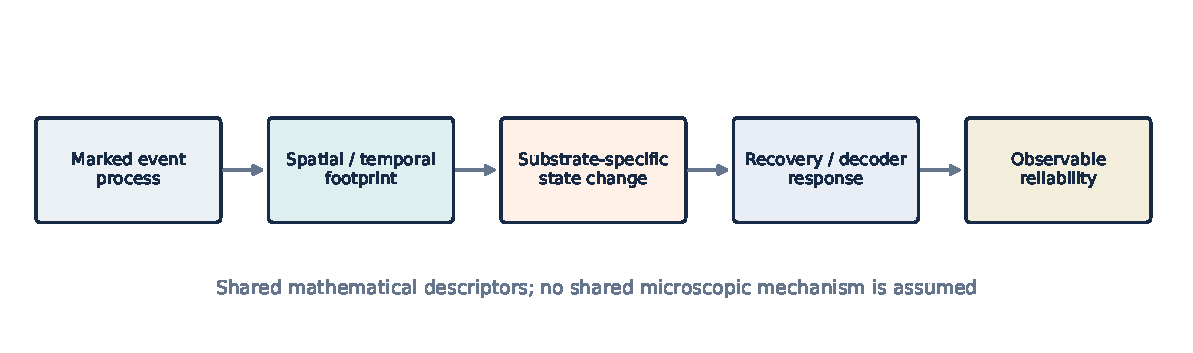
\includegraphics[width=.98\linewidth]{fig01_framework_flow.pdf}\caption{Layered reliability framework. Marked events create domain-specific footprints. The physical or biological substrate map then feeds a code/decoder or repair response. The shared abstraction is the ordering of statistical layers, not a common microscopic process.}\label{fig:framework}\end{figure}

This paper makes six contributions. First, it formalizes a marked space-time representation of disturbance events with geometry and severity marks. Second, it separates event statistics from substrate-specific damage and from recovery capacity. Third, it states queue-stability and Poisson-thinning results with explicit assumptions. Fourth, it proves by a minimal counterexample that equal marginal occupancy does not determine nonlinear failure risk. Fifth, it expands the original finite-lattice experiment with exact expected-occupancy calibration, uncertainty summaries, spatial-correlation and cluster diagnostics, finite-size sensitivity, and track-length sensitivity. Sixth, it specifies quantum and biological experiments that could falsify the proposed model components.

The rest of the paper is organized as follows. Sections~\ref{sec:epistemic}--\ref{sec:radiobio} define the epistemic contract and review the relevant physical domains. Sections~\ref{sec:model}--\ref{sec:theory} develop the common statistical model and its elementary results. Sections~\ref{sec:benchmark}--\ref{sec:results} document the synthetic benchmark. Sections~\ref{sec:translation}--\ref{sec:neutrino} discuss interpretation, measurement design, AI, and the neutrino-fog analogy. Sections~\ref{sec:limitations}--\ref{sec:conclusion} specify limitations, falsification conditions, and conclusions. Appendices provide calibration details, statistical conventions, and a reproducibility protocol.

\section{Epistemic contract and scope of inference}
\label{sec:epistemic}
A long paper can be misleading if the visual scale of the document exceeds the evidential scale of its results. We therefore begin with a scope contract. Statements are divided into four categories: published observations, mathematical consequences of stated assumptions, synthetic outputs from the included code, and proposed experiments. These categories are never merged into a single evidence grade.

\subsection{Published observations}
The quantum-hardware literature establishes that radiation-associated quasiparticle and phonon processes can correlate with qubit errors and coherence changes. Castelli et al. provide detector-synchronized measurements of qubit parameters, while Binney et al. provide a comparative account of radiation and vibration error signatures \citep{Castelli2026,Binney2026}. These are device-specific measurements. They are evidence for structured disturbance channels, not universal material constants and not a measured catastrophic-event probability for a full fault-tolerant computer.

The radiobiology literature establishes that high-LET radiation can generate complex, clustered DNA damage, and that lesion architecture can influence repair kinetics and chromosome-level outcomes \citep{Hagiwara2019,Shibata2022,Goodhead2024,Wilkinson2023}. The 2026 H--Fe simulation database strengthens the availability of species- and energy-dependent track-structure outputs, but a simulation database does not eliminate the need for model validation and uncertainty accounting \citep{Huang2026}.

\subsection{Mathematical consequences}
The queueing and thinning results in Section~\ref{sec:theory} are conditional statements. They follow from assumptions such as Poisson arrivals, independent catastrophic marks, and a single-server workload abstraction. A theorem under a model is not evidence that the model is an adequate representation of a device or cell. In particular, \(\rho<1\) is a stability condition for a specified queue, not a sufficient condition for logical recoverability or cell survival.

\subsection{Synthetic outputs}
The numerical results in this paper come from an idealized finite lattice. Each ``track'' is a finite straight line of lattice sites with a random anchor and one of four orientations. The benchmark counts whether an erased component spans the lattice under four-neighbour connectivity. No charge transport, phonon propagation, syndrome measurement, stabilizer decoding, DNA chemistry, chromatin state, lesion repair enzyme, or cell-fate dynamics is simulated. The benchmark is useful because the dependence structure is transparent and reproducible; its limitations are equally central to the paper.

\subsection{Proposed work}
Calibration from radiation detectors, Geant4 or PARTRAC track structure, quantum hardware, repair microscopy, or biological assays is a future programme. Neural decoders may be trained or adapted to measured event-conditioned noise, but no published decoder is claimed to have already been validated on the exact burst law used here. AlphaQubit 2 is a recent demonstration of scalable real-time neural decoding for topological codes under its evaluated settings; transfer to the radiation-conditioned channel is an open experiment \citep{Senior2025}.

\begin{table}[t]\centering\small\caption{Evidence classes used throughout the manuscript.}\label{tab:evidence}\begin{tabularx}{\linewidth}{p{.18\linewidth}X p{.23\linewidth}}\toprule
Class & What it contains & Permitted inference\\\midrule
Published observation & Device-synchronized radiation measurements; published track-structure and clustered-DNA-damage findings & Evidence in the apparatus, organism, dose, and conditions studied\\
Mathematical result & Queue stability, thinning identities, dependence counterexample & Follows from explicit model assumptions only\\
Synthetic computation & Finite lattice; Poisson line-track generator; Monte Carlo spanning events & Demonstrates properties of the declared surrogate\\
Proposed experiment & Calibrated event maps, code-specific decoding, lesion and repair assays & A test plan, not an achieved result\\\bottomrule\end{tabularx}\end{table}

\begin{scopebox}
No result in the lattice benchmark is called a surface-code threshold, a holographic-code threshold, a DNA damage threshold, a mutation probability, a lifespan estimate, or a biological repair limit. No claim is made that ``one muon defeats a quantum computer.'' No claim is made that solar neutrinos meaningfully damage cellular DNA.
\end{scopebox}

\section{Quantum reliability: radiation, correlated errors, and decoding}
\label{sec:quantum}
\subsection{From radiation events to qubit disturbances}
Ionizing radiation can create energetic phonons and quasiparticles in superconducting substrates and circuit components. Those excitations can propagate and interact with multiple qubits, generating time-correlated error opportunities. The operational measurement is not simply an incoming particle count: it can include detector event times, detector-array coincidence patterns, qubit relaxation times, dephasing metrics, quasiparticle-sensitive observables, and the spatial response across a device. These signals live at different levels of the causal chain and should not be substituted for one another.

Castelli et al. synchronize microwave kinetic-inductance detector arrays with transmon measurements and report statistically significant changes in \(T_1\) and \(T_2\) after selected detected events \citep{Castelli2026}. The result supports the use of event-conditioned covariates. A disciplined statistical analysis would preserve the detector time stamp, coincidence multiplicity, event geometry, measurement latency, device configuration, and competing explanations. The measured percentage change in a coherence parameter is not a logical error rate: a logical rate additionally depends on the code, the decoder, measurement schedule, correlations across cycles, and how often the event occurs.

Binney et al. demonstrate why classification of the disturbance source matters. Radiation-related signatures and pulse-tube vibration signatures can both produce correlated errors, yet have different temporal, spatial, and spectral fingerprints \citep{Binney2026}. A model that labels all correlations as radiation-induced would confound distinct physical processes. The event mark should therefore include source class or a posterior distribution over source classes, and the inference should retain uncertainty in that assignment.

\subsection{From physical faults to a quantum channel}
Let \(\mathcal{H}_P=\bigotimes_{i=1}^{n}\mathcal{H}_i\) denote the physical-qubit Hilbert space and let \(\mathcal{C}\subset\mathcal{H}_P\) be the code subspace. A disturbance event \(z\) induces a quantum channel \(\mathcal{N}_z\) or, in a simplified Pauli description, a distribution over error operators \(E\). A conventional IID model might assign independent error indicators \(X_i\sim\operatorname{Bernoulli}(p)\). A correlated event model instead conditions local error probabilities on a shared random event:
\begin{equation}\label{eq:conditional-error}
\Pp(X_i=1\mid Z=z)=r_i(z),\qquad \Cov(X_i,X_j)=\E[\Cov(X_i,X_j\mid Z)]+\Cov(r_i(Z),r_j(Z)).
\end{equation}
The second covariance term can remain positive even when conditional faults are independent given the event. A shared radiation burst is one possible common cause. This construction is not limited to radiation; vibration, control leakage, thermal excursions, and correlated calibration failures can produce analogous dependence structures.

For a code with distance \(d\), the familiar statement that arbitrary \(t=\lfloor(d-1)/2\rfloor\) errors are correctable is a worst-case combinatorial guarantee, not a prediction for a particular stochastic channel. Under a stochastic channel, logical performance depends on the distribution of error patterns and decoder. Under an erasure channel, the location of each erasure is known to the decoder, and correctability is governed by whether the erased set supports an undetectable logical operator. These are different channel assumptions. Radiation-associated disturbance should not automatically be represented as a known erasure: it may be a mixture of dephasing, relaxation, leakage, measurement faults, and burst-induced correlations.

\subsection{Why correlations matter to decoders}
A decoder that assumes factorized likelihoods may score a correlated event as many independent faults. The same total number of single-qubit error indicators can produce radically different geometry depending on where those errors land. If a cluster aligns with a logical operator or creates an ambiguous syndrome history, a code may fail at a rate not predicted by mean occupancy alone. Conversely, a decoder that knows the event-conditioned likelihood may exploit the structure and improve performance, provided the event model is calibrated and the decoder can process the information within the cycle deadline.

A relevant operational metric is a logical failure probability per round, \(p_L(d,\eta,\tau)\), conditioned on code distance \(d\), channel parameters \(\eta\), and decoder latency budget \(\tau\). Another is the probability that a radiation event generates a correlated fault pattern outside a decoder's modeled support. The appropriate benchmark compares independent and burst channels at matched marginal rates, the same code, the same decoder, identical measurement schedule, equal latency constraints, and held-out event traces. If event detection is used as side information, the detector latency and false-positive/false-negative rates must also be included.

\subsection{Holographic quantum error correction: a code-theoretic lens}
Holographic codes provide a particularly useful example of geometry-dependent recoverability. Tensor-network constructions encode bulk logical degrees of freedom into boundary degrees of freedom, and can represent reconstruction of a logical operator on different boundary regions. The original HaPPY construction makes this relation explicit in a family of toy models \citep{Pastawski2015}. Harlow showed how quantum error-correction language explains a version of the Ryu--Takayanagi relation and entanglement-wedge reconstruction \citep{Harlow2017}. Later CSS holographic codes and threshold analyses have developed the code family and its erasure properties \citep{Harris2018,Bao2022}.

For a specified encoding isometry \(V:\mathcal{H}_L\rightarrow\mathcal{H}_P\) and erased boundary subset \(E\), exact erasure correction of a logical subsystem can be expressed through the Knill--Laflamme condition. If \(P=VV^\dagger\) is the code projector and \(\{E_a\}\) spans the error set supported on \(E\), then
\begin{equation}\label{eq:KL}
P E_a^\dagger E_b P = c_{ab}P \quad \text{for all }a,b.
\end{equation}
For erasures, the locations are known and the condition can be recast through decoupling of the erased region from the logical subsystem. In holographic settings, reconstruction regions and entanglement wedges depend on the code geometry and selected logical algebra. The existence of a holographic code does not confer a universal tolerance to arbitrary extended bursts. A burst must be mapped onto the code's physical boundary degrees of freedom and tested against the code-specific erasure or general-noise correctability condition.

A physically honest project would instantiate at least one explicit code family, publish its tensors or stabilizers, define the boundary placement of the physical qubits, construct burst-conditioned channels, run the decoder, and measure logical failure and decoding time over code sizes. The lattice experiment in this manuscript performs none of those code-specific steps. It offers a geometric warning that an equal-occupancy comparison can conceal major differences in cluster structure; it is not a holographic threshold calculation.

\begin{figure}[t]\centering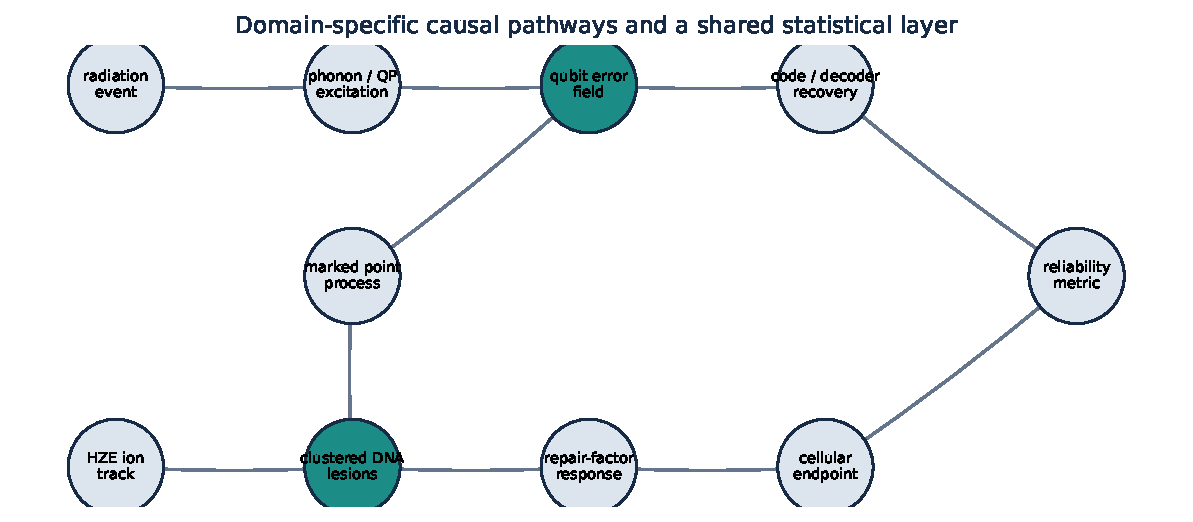
\includegraphics[width=.95\linewidth]{fig02_domain_causal_graph.pdf}\caption{Causal layers across the two domains. The shared marked-event process supplies statistical structure; the quantum and biological causal branches remain different. A dashed conceptual bridge is represented through the common reliability metric, not through identical state dynamics.}\label{fig:domain-graph}\end{figure}

\section{Radiobiology: high-LET tracks and clustered lesions}
\label{sec:radiobio}
\subsection{Track structure is more informative than dose alone}
Absorbed dose is an energy-per-mass summary. It is an essential exposure quantity, but it does not uniquely specify the nanoscale or microscale spatial organization of energy deposition. High-LET charged particles deposit energy densely along tracks. Depending on species, energy, geometry, cell state, and chromatin context, the resulting damage can include single-strand breaks, double-strand breaks, base damage, chemically complex lesions, and clusters of lesions separated by short distances \citep{Hagiwara2019,Shibata2022,Goodhead2024,Wilkinson2023}.

The scale of lesion complexity matters. A locally dense cluster may require coordinated processing and can pose different risks than the same count of isolated lesions. But a lesion cluster is not equivalent to an unrepaired break, and an unrepaired break is not equivalent to mutation, chromosome aberration, or cell death. Each endpoint has a separate measurement definition and time scale. A model that collapses all endpoints into a single binary ``cell failed'' label discards the causal sequence that experiments are intended to resolve.

Hagiwara et al. review the formation of clustered double-strand breaks and repair following heavy-ion irradiation, including chromosome-scale outcomes and lesion organization \citep{Hagiwara2019}. Shibata reviews clustered DNA damage following carbon-ion irradiation and the influence of LET and lesion complexity \citep{Shibata2022}. Goodhead and Weinfeld trace the development of the clustered-damage concept across physics, chemistry, and cellular response \citep{Goodhead2024}. Wilkinson, Hill, and Parsons review cellular responses to complex radiation-induced DNA damage \citep{Wilkinson2023}. Together, these works justify retaining a spatial damage representation. They do not justify treating all tracks as equivalent or assigning one repair workload to each particle.

\subsection{Track-structure data and model calibration}
Recent H--Fe track-structure simulations provide a useful resource for species- and energy-dependent DNA damage distributions \citep{Huang2026}. Such data can inform mark distributions: LET, radial dose, track radius, secondary-electron structure, lesion multiplicity, cluster density, and energy. A calibrated model should preserve the distinction between physical track variables and biological response variables. For example, a radial dose kernel is not itself a double-strand-break probability; chemistry and chromatin determine how energy deposition becomes a lesion endpoint.

A generic spatial lesion field can be written as
\begin{equation}\label{eq:lesion-field}
L(x,t)=\sum_k W_k K_{\ell}\!\left(x-X_k;\Theta_k,\Lambda_k\right)G_k(t-T_k),
\end{equation}
where \(K_\ell\) is a domain-specific spatial kernel, \(W_k\) represents severity or expected lesion workload, \(\Theta_k\) includes orientation and radiation quality, \(\Lambda_k\) includes track scale, and \(G_k\) describes temporal chemistry or processing. The choice of threshold for calling a lesion cluster must be tied to an assay and genomic scale. A point-process kernel used for a synthetic lattice is not an empirically calibrated DNA lesion kernel.

\subsection{A controllable perturbation is not a physical substitute}
House et al. developed a dCas9--KillerRed system that can generate transient, localized, light-activated oxidative DNA damage at targeted genomic regions. Their study reports site-specific oxidative damage, rapid repair under tested conditions, and few detectable sequencing errors in that experimental context \citep{House2020}. The system is valuable because it can help study local repair kinetics and perturb genomic regions in a controlled manner. It is not a high-LET heavy-ion track, does not reproduce the full secondary-particle and energy-deposition structure of an HZE ion, and is not evidence that targeted damage inevitably overwhelms repair.

The 2025 review by Dey and Barnes surveys genetically targeted oxidative-stress approaches and helps place such tools within a broader perturbation landscape \citep{Dey2025}. For any experimental use, light dose, guide specificity, KillerRed expression, oxygen availability, local ROS chemistry, off-target effects, repair pathway, and assay sensitivity would need explicit controls. A benchmark must also distinguish initial damage induction from persistence of damage and from downstream functional effects.

\section{A shared mathematical language without a shared mechanism}
\label{sec:model}
\subsection{Marked space-time events}
Let \((\Omega,\mathcal{F},\Pp)\) be a probability space. A disturbance history is represented by a marked point process
\begin{equation}\label{eq:point-process}
\Phi=\sum_{k}\delta_{Z_k},\qquad Z_k=(T_k,X_k,\Theta_k,L_k,W_k,M_k).
\end{equation}
Here \(T_k\) is event time, \(X_k\) is an anchor location, \(\Theta_k\) describes orientation or morphology, \(L_k\) is an extent or scale parameter, \(W_k\) is severity or workload, and \(M_k\) is a source or mechanism mark. The location space may be a device graph, a two-dimensional chip layout, a three-dimensional cell nucleus, or a genomic coordinate system. Time may be continuous, discrete, or a mixed event/cycle index.

The event process can be homogeneous Poisson, inhomogeneous Poisson, Cox, Hawkes, renewal, or a physically specified transport-derived process. A homogeneous Poisson process is an analytically convenient baseline, not a claim that cosmic-ray events or DNA lesions are universally Poisson in every observed coordinate. Event clustering can arise from parent-child processes, latent environmental fluctuations, or a common physical event that generates a multi-site footprint. The model class should be selected from detector and assay data rather than from mathematical convenience alone \citep{LastPenrose2017,MollerWaagepetersen2004}.

\subsection{Footprints and local burden}
For event mark \(z\), define a spatial footprint \(C(z)\subseteq\cX\) or a nonnegative kernel \(K(x;z)\). In a binary model, the damaged region at time \(t\) is
\begin{equation}\label{eq:damage-union}
D_t=\bigcup_{k:T_k\le t} C(Z_k),
\end{equation}
possibly after applying a persistence or recovery rule. In a soft-burden model,
\begin{equation}\label{eq:burden}
B(x,t)=\sum_{k:T_k\le t} W_k K(x-X_k;\Theta_k,L_k)G(t-T_k;Z_k).
\end{equation}
A binary state can be derived by thresholding \(B\), but preserving the continuous field is often preferable because the threshold can be assay-dependent and multiple weak exposures may accumulate.

The footprint need not be a contiguous disk or line. A quantum event may induce a device-specific correlated error map through a phonon/quasiparticle propagator; a charged-particle track may induce a narrow core plus a radial halo of secondary-electron damage. The same abstract mark tuple does not force identical kernels. In fact, the most important domain-specific work is usually the estimation of \(K\), \(G\), and the conditional map from physical event to observable disturbance.

\subsection{Substrate maps}
For a quantum device, let \(\mathfrak{Q}\) map a realization of \(\Phi\) into a quantum channel history \(\mathcal{N}_{0:H}\), potentially including Pauli faults, leakage, amplitude damping, correlated measurement errors, and non-Markovian memory. For a cell, let \(\mathfrak{B}\) map \(\Phi\) into a lesion process, repair-factor response, chromatin state, and downstream endpoint. The common notation is
\begin{equation}\label{eq:substrate-map}
\Phi\xrightarrow{\mathfrak{Q}}\mathcal{N}_{0:H}\xrightarrow{\mathfrak{D}}\text{logical outcome},\qquad
\Phi\xrightarrow{\mathfrak{B}}L_{0:H}\xrightarrow{\mathfrak{R}}\text{biological endpoint}.
\end{equation}
The maps \(\mathfrak{Q}\), \(\mathfrak{B}\), \(\mathfrak{D}\), and \(\mathfrak{R}\) have separate parameters, validation standards, and failure definitions.

\subsection{Observable-specific failure}
Let \(Y_Q\) denote a quantum logical observable, such as a logical Pauli error in one correction cycle or a logical failure during a fixed algorithmic horizon. Let \(Y_B\) denote a biological endpoint, such as persistent clustered lesions at time \(\tau\), chromosome aberration frequency, mutation burden, clonogenic survival, or a defined functional phenotype. A generic reliability event is
\begin{equation}\label{eq:failure}
F_Q=\{Y_Q\in\cF_Q\},\qquad F_B=\{Y_B\in\cF_B\}.
\end{equation}
The failure sets are not interchangeable. A comparison is meaningful only at the level of shared statistical descriptors, not by equating \(F_Q\) and \(F_B\).

\begin{table}[t]\centering\small\caption{Correspondence between statistical abstractions and domain-specific quantities.}\label{tab:correspondence}\begin{tabularx}{\linewidth}{p{.2\linewidth}XX}\toprule
Abstract object & Quantum device interpretation & Cellular/radiobiology interpretation\\\midrule
Event time \(T_k\) & Radiation detector event or burst onset & Particle traversal / energy-deposition event\\
Anchor \(X_k\) & Chip coordinate or phonon-origin region & Nuclear or chromatin coordinate\\
Orientation \(\Theta_k\) & Device geometry, propagation direction, anisotropic response & Particle-track direction and local geometry\\
Extent \(L_k\) & Correlation length/time of device response & Track length, radial scale, lesion-cluster extent\\
Severity \(W_k\) & Conditional channel strength, leakage or fault weight & Lesion multiplicity / complexity or repair workload proxy\\
Recovery map & Syndrome extraction, decoder and logical recovery & Repair pathways, checkpoints, chromatin and cell response\\
Failure observable & Logical error, loss of state fidelity, deadline miss & Persistent lesion, aberration, mutation, loss of viability\\\bottomrule\end{tabularx}\end{table}

\section{Recovery as a finite-capacity process}
\label{sec:recovery}
\subsection{Quantum recovery is not a single-server queue}
A quantum decoder consumes measurement outcomes and produces corrections or Pauli-frame updates. Its workload can include syndrome processing, belief updates, neural inference, communication, and memory movement. The cycle deadline is a real-time constraint: even an accurate correction may be operationally too late if it arrives after the control system requires it. Nevertheless, quantum recovery is not generally reducible to one scalar repair server. A queue is at most a useful abstraction for a chosen processing subsystem, such as a decoder pipeline or a finite bandwidth path for event metadata.

For a code, recoverability is first a channel-and-code property. The decoder then approximates or implements an optimal or near-optimal inference rule under the supplied noise model. The performance metrics include logical failure probability, decoding latency, throughput, memory use, and degradation under distribution shift. A decoder trained on independent depolarizing noise may be miscalibrated under rare correlated bursts even if the marginal single-qubit error rate is unchanged.

\subsection{Biological repair workload}
DNA repair is distributed across multiple molecular pathways and regulated by cell state. A lesion may be recognized, processed, resected, ligated, bypassed, or left persistent; pathway use can depend on lesion chemistry, cell-cycle phase, chromatin accessibility, and local protein availability. A scalar service capacity \(\mu\) therefore cannot represent the whole biological response. It can be a coarse aggregate for a restricted assay or a theoretical workload variable, provided its interpretation is declared and measured.

Define a repair-workload unit as an empirically calibrated quantity of pathway-specific processing demand. For example, an assay might estimate expected repair-factor occupancy time per lesion class, or infer a distribution of processing time for a defined lesion type under a specified cell condition. A single heavy-ion event may generate a random total workload \(S_k\), with distribution depending on LET, species, cell state, and cluster architecture. If repair capacity varies over time, write \(\mu(t)\). If multiple pathways operate in parallel, the model requires a service network or vector capacity \(\boldsymbol{\mu}\), not a scalar.

\subsection{Lindley workload recursion}
For a restricted single-server abstraction, let \(A_n\) be the interarrival time between event workloads, let \(S_n\) be service work, and let \(\mu\) be constant service capacity measured in work units per unit time. The unfinished work immediately before event \(n\) obeys
\begin{equation}\label{eq:lindley}
W_{n+1}=\max\{0,\,W_n+S_n-\mu A_{n+1}\}.
\end{equation}
This recursion is useful because it makes recovery debt explicit. When event spacing is long relative to service demand, the queue empties. When multiple large workloads arrive close together, unfinished work accumulates. The recurrence also clarifies why identical event counts can have different outcomes: the order and spacing of workloads matter.

A continuous-time M/G/1 approximation has Poisson arrivals at rate \(\lambda\), independent identically distributed service requirements \(S\), and constant service rate \(\mu\). Its traffic intensity is
\begin{equation}\label{eq:rho}
\rho=\frac{\lambda\E[S]}{\mu}.
\end{equation}
The condition \(\rho<1\) is the standard stability condition for this model. It is not a sufficient condition for every lesion to be repaired before a biological checkpoint, nor for every quantum fault to be decoded before a deadline. It says that the long-run offered workload is below mean service capacity in the specified queue.

\begin{table}[t]\centering\small\caption{Recovery metrics that must remain distinct.}\label{tab:recovery-metrics}\begin{tabularx}{\linewidth}{p{.23\linewidth}XX}\toprule
Metric & Quantum system & Biological system\\\midrule
Correctability & Whether an error set is correctable for a code & No direct analogue; lesion processing depends on molecular context\\
Inference/processing delay & Decoder latency per cycle or event & Repair-factor recruitment and processing times\\
Workload accumulation & Queue in a decoder or control pipeline & Unfinished lesion-processing demand under selected pathway abstraction\\
Failure endpoint & Logical error, leaked state, cycle deadline miss & Persistent lesion, aberration, mutation, loss of viability\\
Recovery reserve & Redundancy, code distance, decoder throughput & Repair pathway availability, checkpoint capacity, chromatin context\\\bottomrule\end{tabularx}\end{table}

\section{Theory: dependence, workload stability, and horizon risk}
\label{sec:theory}
\subsection{Equal marginals do not determine joint failure risk}
An average occupancy statistic can conceal radically different dependence structures. The following proposition is elementary, but it is a useful guardrail for all matched-rate comparisons.

\begin{proposition}[Two-site dependence counterexample]\label{prop:dependence}
Consider a system that fails if both of two sites are disturbed. Let each site have marginal disturbance probability \(p\in(0,1)\). Under independent disturbances, the failure probability is \(p^2\). Under a common-shock model in which both sites are disturbed together with probability \(p\), the marginal probabilities are still \(p\), but the failure probability is \(p\). Thus equal marginals do not determine the failure probability.
\end{proposition}
\begin{proof}
For independent Bernoulli indicators \(X_1,X_2\), \(\Pp(X_1=X_2=1)=\Pp(X_1=1)\Pp(X_2=1)=p^2\). Under the common-shock construction, set \(X_1=X_2=U\) where \(U\sim\operatorname{Bernoulli}(p)\). Each marginal remains \(p\), while \(\Pp(X_1=X_2=1)=\Pp(U=1)=p\). Since \(p^2\ne p\) for \(p\in(0,1)\), the failure probabilities differ.\end{proof}

This result does not say that positive correlation always increases every conceivable failure event. The direction depends on the event geometry, code, and observable. It says that marginal calibration alone does not identify a nonlinear failure functional. A matched-occupancy experiment must either measure relevant dependence statistics or state that its comparison is one particular channel contrast.

\subsection{Queue stability result}
\begin{proposition}[M/G/1 workload stability]\label{prop:queue}
Assume Poisson arrivals with rate \(\lambda>0\), iid nonnegative service requirements \(S_k\) with finite mean, a work-conserving single server with constant service rate \(\mu>0\), and no abandonment or feedback. The standard M/G/1 workload process admits a proper stationary workload distribution when \(\rho=\lambda\E[S]/\mu<1\). When \(\rho\ge1\), the offered work is not below service capacity and a finite stationary workload distribution does not exist under the usual nondegenerate assumptions.
\end{proposition}
\begin{proof}
Rescale service work into time units by defining \(B=S/\mu\). The server then has unit service speed and the M/G/1 traffic intensity is \(\lambda\E[B]=\lambda\E[S]/\mu=\rho\). The classical M/G/1 stability criterion is \(\rho<1\), under the stated finite-mean assumptions. The proposition is the workload version of this standard result; see, for example, \citet{GrossHarris1998}.\end{proof}

For heavy-tailed workloads, the queue can be stable while its stationary workload has a long tail and large quantiles. A finite mean does not guarantee a small probability of severe backlog. A practical study should estimate not only \(\E[S]\), but also the tail, variance, possible mixture structure, and dependence of workload on prior events. If events arrive in clusters or if service capacity changes with time, the M/G/1 criterion is no longer automatically sufficient. A Markov-modulated, batch-arrival, or network-of-queues model may be required.

\subsection{Catastrophic marked-event risk}
Suppose disturbance arrivals are Poisson with rate \(\lambda\). Each arrival independently receives a mark and is catastrophic with probability \(q_F\), where catastrophe is defined relative to a specified code/decoder or biological endpoint. Independent thinning implies that catastrophic events form a Poisson process with rate \(\lambda q_F\).

\begin{proposition}[Poisson thinning horizon risk]\label{prop:thinning}
Under the preceding assumptions, the probability of at least one catastrophic event in a horizon of length \(T\ge0\) is
\begin{equation}\label{eq:catrisk}
P_{\mathrm{cat}}(T)=1-\exp(-\lambda q_F T).
\end{equation}
\end{proposition}
\begin{proof}
The count of arrivals in the horizon is Poisson with mean \(\lambda T\). Independent marking retains each event with probability \(q_F\), so the retained count is Poisson with mean \(\lambda q_F T\). The probability of zero retained events is \(\exp(-\lambda q_F T)\); its complement yields the result.\end{proof}

The quantity \(q_F\) is not a universal constant. It depends on the code or biological system, the event mark distribution, operating conditions, recovery response, and chosen endpoint. For quantum hardware, it could be the conditional probability that a radiation event drives a logical failure within a specified correction horizon. For a cell, it could be the probability that the event causes a chosen biological endpoint under specified exposure and repair conditions. Those probabilities must be separately measured.

\subsection{A model-conditional risk envelope}
For a target horizon risk \(\epsilon\in(0,1)\), Equation~\eqref{eq:catrisk} implies
\begin{equation}\label{eq:risk-envelope}
\lambda q_F \leq \frac{-\log(1-\epsilon)}{T}.
\end{equation}
Combining this with queue stability gives two distinct constraints: one on the expected workload offered to a recovery process and one on the rate of events that individually cross a declared catastrophic boundary. Neither constraint subsumes the other. A system can have \(\rho<1\) but still experience rare catastrophic events; conversely, an individual event may be non-catastrophic while the long-run workload is unstable.

\begin{resultbox}
The safe operating region is a function of at least the event rate, the full mark distribution, footprint law, code or repair model, finite recovery capacity, observation horizon, and the acceptable risk. No universal scalar ``burst threshold'' follows from average occupancy or dose alone.
\end{resultbox}

\subsection{Dimensionless descriptors for cross-domain comparison}
Useful comparisons can be organized around dimensionless ratios, provided their domain-specific interpretation is preserved. Examples include the expected number of events per recovery time \(\lambda\tau_R\), burst extent relative to code distance or characteristic repair-domain size \(L/d\) or \(L/\ell_R\), offered workload ratio \(\rho\), and the number of correlated sites per event divided by the number of active components. These ratios do not create a common physical unit. They help compare structural regimes such as isolated disturbances, overlapping bursts, and recovery backlog.

\section{Benchmark design: a transparent geometric surrogate}
\label{sec:benchmark}
\subsection{Why a surrogate is used}
A physical quantum-code simulation and a biological track-structure simulation require different toolchains, parameter sets, and validation data. A surface-code study requires a specific stabilizer layout, measurement circuit, detector error model, decoder, and finite-size scaling. A radiobiology study requires physical track transport and chemical/biological response models. The present experiment isolates a narrower mathematical question: can two channels with the same expected lattice-wide mean occupancy have different spanning-connectivity statistics when one channel has spatially correlated finite footprints?

The lattice is a finite square graph \(G_N=(V_N,E_N)\) with \(N\times N\) sites and four-neighbour edges. A site is declared erased or occupied by a disturbance. Failure is defined as the existence of a four-neighbour connected component touching opposite boundaries, either left-to-right or bottom-to-top. This event is a deliberately simple geometric proxy for a connected failure set; it is not an encoded logical failure.

\subsection{IID channel}
For target probability \(p\), each lattice site is independently erased with probability \(p\):
\begin{equation}\label{eq:iid}
X_i\overset{\mathrm{iid}}{\sim}\operatorname{Bernoulli}(p),\qquad i\in V_N.
\end{equation}
This is a homogeneous baseline with identical sitewise marginals and no spatial covariance between distinct sites.

\subsection{Finite-track channel}
A track is a straight segment of five lattice sites centered at a uniformly selected anchor and oriented uniformly among four directions: horizontal, vertical, and the two diagonals. A Poisson number of tracks is superposed on the lattice. Tracks are clipped at boundaries; if several tracks cover the same site, it is still counted once. Let \(q_i\) denote the probability that one uniformly anchored and oriented track covers site \(i\). For a Poisson number of independent track placements with intensity \(\lambda_T\), Poisson thinning gives
\begin{equation}\label{eq:sitehit}
\Pp(X_i=1)=1-\exp(-\lambda_Tq_i).
\end{equation}
Because tracks are clipped, the \(q_i\) values are not constant across the lattice. The calibration target is not site-by-site equality with the IID model. It is exact equality of expected lattice-wide mean occupancy:
\begin{equation}\label{eq:calibration}
\frac{1}{N^2}\sum_{i\in V_N}\left[1-\exp(-\lambda_Tq_i)\right]=p.
\end{equation}
The unique nonnegative solution is found by bisection because the left side is continuous and strictly increasing in \(\lambda_T\) whenever at least one site has positive hit probability. Appendix~\ref{app:calibration} gives the computation and boundary discussion.

\subsection{Simulation protocol}
The primary experiment uses \(N=24\), ten probability values from 0.20 to 0.65 in increments of 0.05, 4,000 trials per channel at each probability, and random seed 20261106. One generator produces the IID mask and then the track mask for each trial. The main benchmark records the number of spanning masks. A separate sensitivity analysis uses lattice sizes 12, 18, 24, and 32 with 700 trials per probability and channel at \(p\in\{0.30,0.40,0.50\}\). A second sensitivity analysis varies track length among 3, 5, and 7 sites, using 900 trials per probability and track length at \(p\in\{0.30,0.40,0.50\}\). These additional sweeps are explicitly labelled diagnostic simulations, not evidence for a physical scaling law.

\begin{figure}[t]\centering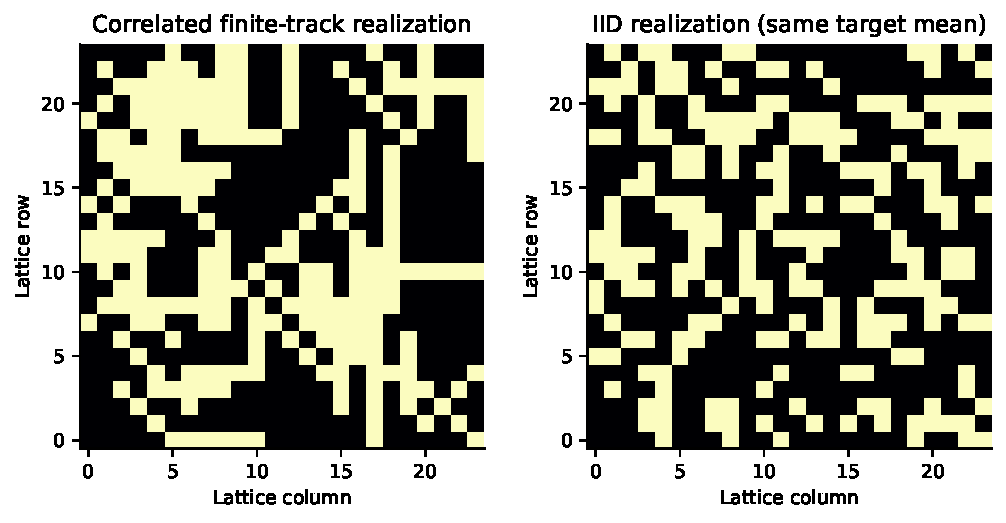
\includegraphics[width=.94\linewidth]{fig03_spatial_realizations.pdf}\caption{Illustrative independent and correlated masks with the same target lattice-wide mean occupancy. Individual realizations fluctuate, and the track process has edge-dependent sitewise marginals due to clipping. The figure illustrates channel geometry rather than physical radiation tracks.}\label{fig:realizations}\end{figure}

\begin{table}[t]\centering\small\caption{Primary synthetic benchmark specification.}\label{tab:benchmark-spec}\begin{tabularx}{\linewidth}{p{.29\linewidth}X}\toprule
Component & Declared specification\\\midrule
Graph & Square lattice, \(N=24\), four-neighbour adjacency\\
Failure event & Any erased component spans left--right or bottom--top\\
IID process & Independent Bernoulli occupancy with probability \(p\)\\
Track process & Poisson count; uniform anchor; four equally likely orientations; five-site straight segment; clipped at boundary\\
Calibration & Bisection solving the exact expected lattice-wide mean occupancy equation\\
Probability grid & 0.20, 0.25, \ldots, 0.65 (ten points)\\
Monte Carlo & 4,000 trials per channel and probability; seed 20261106\\
Inference & Frequencies with Wilson 95\% intervals; no claim of asymptotic threshold\\\bottomrule\end{tabularx}\end{table}

\subsection{Uncertainty convention}
For a count \(k\) in \(n\) Bernoulli trials, the sample rate is \(\hat p=k/n\). We report Wilson score intervals with the 1.96 normal quantile. A zero count is not interpreted as zero probability. At \(k=0,n=4,000\), the rough rule-of-three upper bound is \(3/4,000=0.00075\), or 0.075\%. The Wilson interval used by the code is also nonzero. The intervals represent Monte Carlo uncertainty under the synthetic generator; they do not include model uncertainty, physical calibration error, or uncertainty about whether the surrogate is appropriate.

\section{Benchmark results}
\label{sec:results}
\subsection{Primary spanning frequencies}
Table~\ref{tab:main-results} gives the primary outcomes. The track channel has a higher observed spanning frequency at every one of the ten tested grid points. At \(p=0.40\), the IID channel produced 0 spanning masks in 4,000 trials, while the track process produced 705, a frequency of 17.625\%. At \(p=0.50\), the rates were 5.475\% and 68.425\%. At \(p=0.60\), the rates were 74.300\% and 96.900\%. This pattern is a property of the selected finite lattice, track geometry, boundary rule, and spanning definition.

\begin{table}[H]\centering\small\caption{Primary 24\(\times\)24 benchmark: spanning failures in 4,000 trials per channel.}\label{tab:main-results}\begin{tabular}{rrrrr}\toprule
Target \(p\) & IID failures & Track failures & IID rate & Track rate\\\midrule
0.20 & 0 & 2 & 0.000\% & 0.050\%\\
0.25 & 0 & 7 & 0.000\% & 0.175\%\\
0.30 & 0 & 45 & 0.000\% & 1.125\%\\
0.35 & 0 & 224 & 0.000\% & 5.600\%\\
0.40 & 0 & 705 & 0.000\% & 17.625\%\\
0.45 & 11 & 1,606 & 0.275\% & 40.150\%\\
0.50 & 219 & 2,737 & 5.475\% & 68.425\%\\
0.55 & 1,229 & 3,497 & 30.725\% & 87.425\%\\
0.60 & 2,972 & 3,876 & 74.300\% & 96.900\%\\
0.65 & 3,893 & 3,984 & 97.325\% & 99.600\%\\\bottomrule\end{tabular}\end{table}

The curve in Figure~\ref{fig:spanning} visualizes these results with Wilson intervals. At low occupancy, the absolute failure rate is small in both channels, but the track channel begins producing spanning events earlier in the tested grid. At high occupancy, both channels approach saturation. The visual gap is largest in the intermediate regime where connectivity is sensitive to cluster geometry. This shape should not be mistaken for a sharp thermodynamic phase transition: the lattice has finite size, the channel has a fixed synthetic track law, and the sweep samples only ten discrete probabilities.

\begin{figure}[t]\centering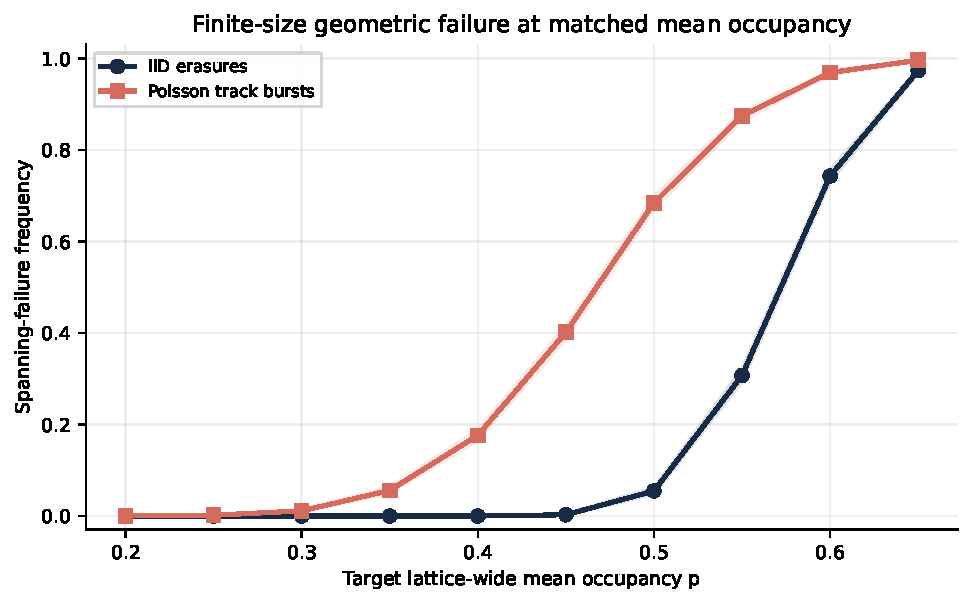
\includegraphics[width=.92\linewidth]{fig04_spanning_failure_curve.pdf}\caption{Primary Monte Carlo spanning frequencies with Wilson 95\% intervals. The figure compares two synthetic channels at matched expected lattice-wide mean occupancy. It is not a physical threshold curve.}\label{fig:spanning}\end{figure}

\subsection{Spatial covariance and component-size distribution}
The track process induces positive spatial covariance for nearby sites because one track can cover more than one site. Figure~\ref{fig:covariance} plots the mean covariance for horizontal separations. The covariance decays with separation in this finite straight-line model because a single short track is less likely to cover both sites when they are farther apart. Orientation and boundary clipping create anisotropy that a radial average would conceal. The diagnostic therefore reports horizontal separations only and is not presented as an isotropic correlation function.

\begin{figure}[t]\centering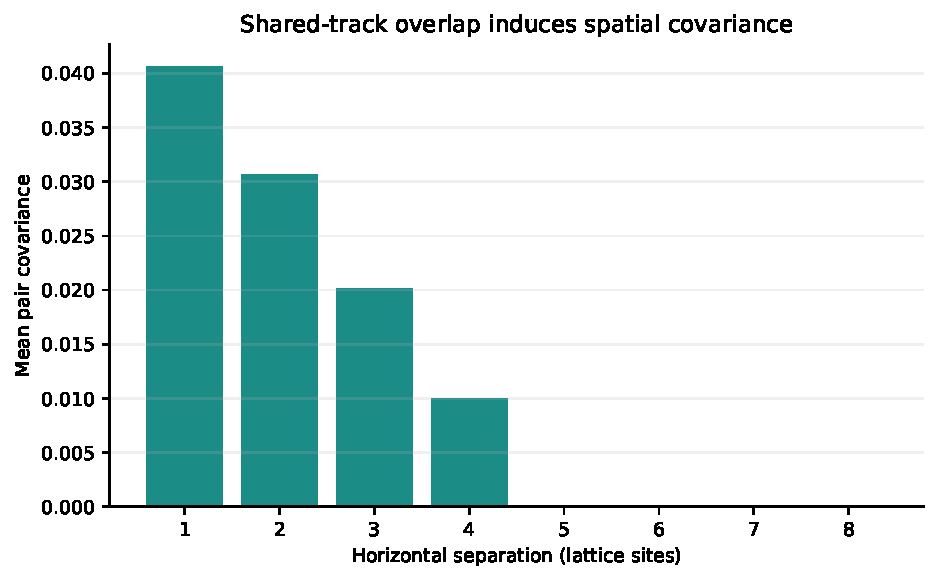
\includegraphics[width=.82\linewidth]{fig05_pair_covariance.pdf}\caption{Analytic mean pair covariance under the Poisson track model at target occupancy \(p=0.40\). The values follow from exact shared-track coverage probabilities for horizontal pairs; they are not fitted to radiation data.}\label{fig:covariance}\end{figure}

Figure~\ref{fig:clusters} shows the distribution of sizes of four-neighbour erased components from 1,600 additional realizations per channel at target occupancy \(p=0.40\). The comparison is descriptive. It reveals how the dependence law changes the component-size distribution even when the mean occupancy target is the same. The tail of the cluster-size distribution matters for spanning risk, but the histogram does not itself define logical failure for a quantum code or unrepaired damage for a cell.

\begin{figure}[t]\centering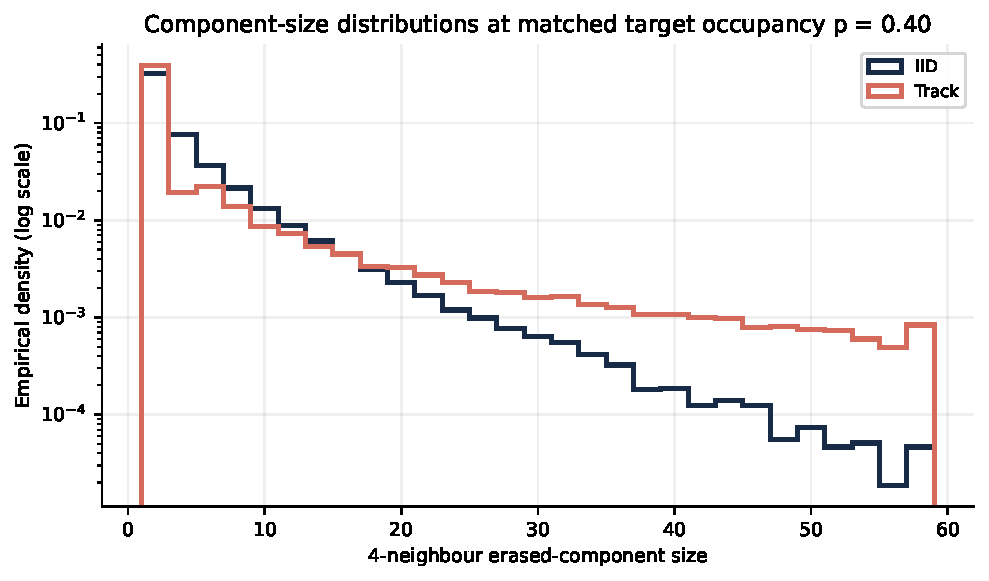
\includegraphics[width=.88\linewidth]{fig06_cluster_size_distribution.pdf}\caption{Empirical distribution of 4-neighbour erased-component sizes at matched target occupancy \(p=0.40\). The logarithmic vertical scale emphasizes the tail.}\label{fig:clusters}\end{figure}

\subsection{Finite-size sensitivity}
A finite-size experiment asks whether the qualitative relationship persists as the graph changes. Figure~\ref{fig:finitesize} summarizes simulations at lattice sides \(N=12,18,24,32\), with 700 trials per point for three probabilities. The observed values fluctuate because the number of trials is finite. The curves are not sufficient for finite-size scaling exponents or a critical threshold estimate. A credible threshold study would require more sizes, denser sampling near the transition, uncertainty propagation, a documented scaling ansatz, and independent validation of the channel law.

\begin{figure}[t]\centering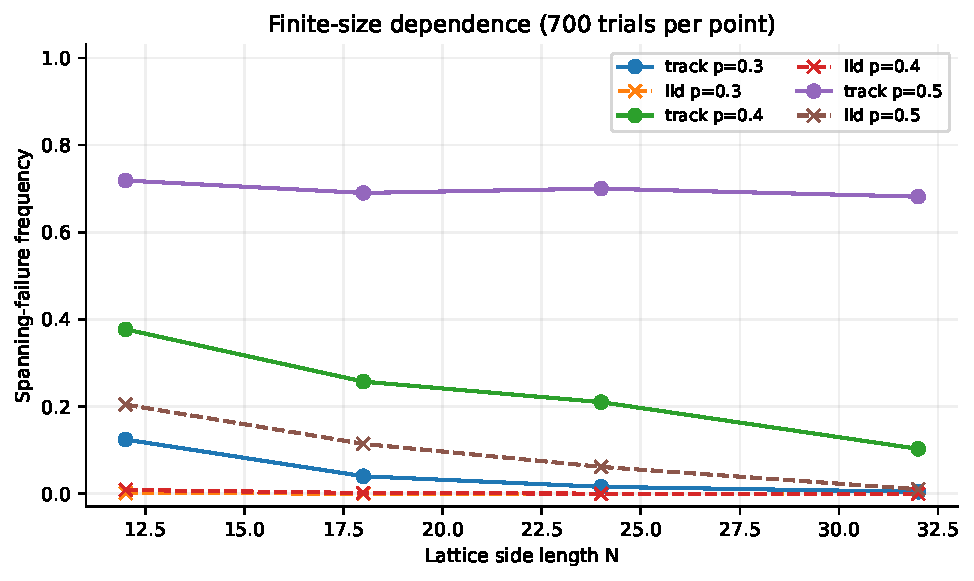
\includegraphics[width=.92\linewidth]{fig07_finite_size_sensitivity.pdf}\caption{Finite-size sensitivity for three occupancy values. Each point uses 700 trials per channel. The panel is a diagnostic of the chosen surrogate, not a finite-size scaling analysis of a quantum code.}\label{fig:finitesize}\end{figure}

\subsection{Binomial uncertainty}
Figure~\ref{fig:uncertainty} compares intervals for \(p=0.40,0.50,0.60\). When the IID count is zero, the lower end is zero and the upper end remains positive. This is important because reporting ``0\%'' without a sample-size statement can create a false sense of certainty. For the track channel, the intervals are narrow relative to the observed differences because 4,000 trials are used, but they still quantify only Monte Carlo sampling error.

\begin{figure}[t]\centering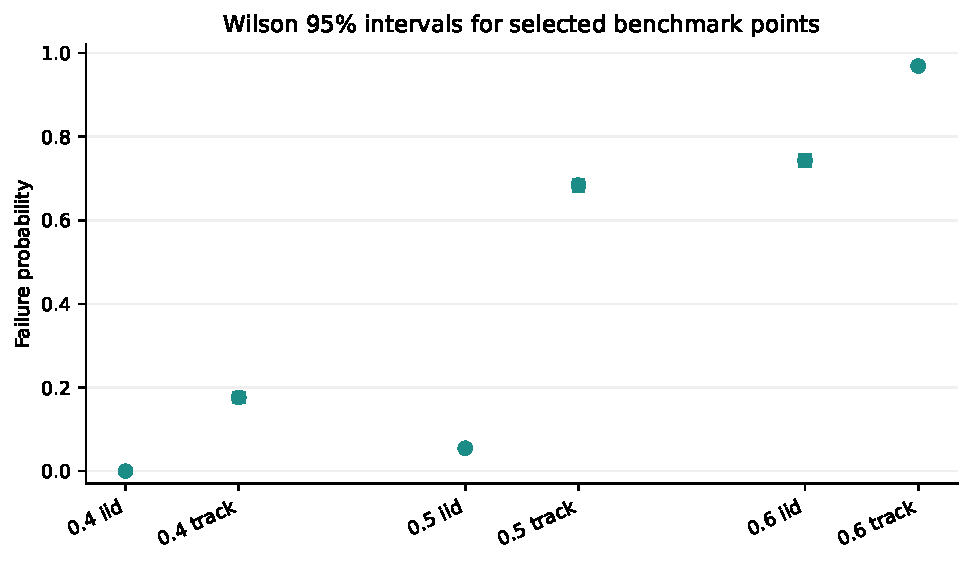
\includegraphics[width=.88\linewidth]{fig08_binomial_uncertainty.pdf}\caption{Wilson 95\% intervals for selected primary benchmark points. The zero-failure IID observations at \(p=0.40\) and below have nonzero upper confidence limits.}\label{fig:uncertainty}\end{figure}

\subsection{Track-length sensitivity}
A key model assumption is the five-site track length. The sensitivity analysis changes the segment length to 3 and 7 sites, recalibrating the Poisson intensity separately so that expected lattice-wide mean occupancy remains fixed. Figure~\ref{fig:length} displays the resulting track-channel spanning frequencies. The analysis illustrates that track morphology is not a nuisance parameter that can be omitted: longer segments tend to create different connected components, while exact direction, clipping, and anchor statistics also matter. The finite Monte Carlo values should not be extrapolated to a real ion track without physical calibration.

\begin{figure}[t]\centering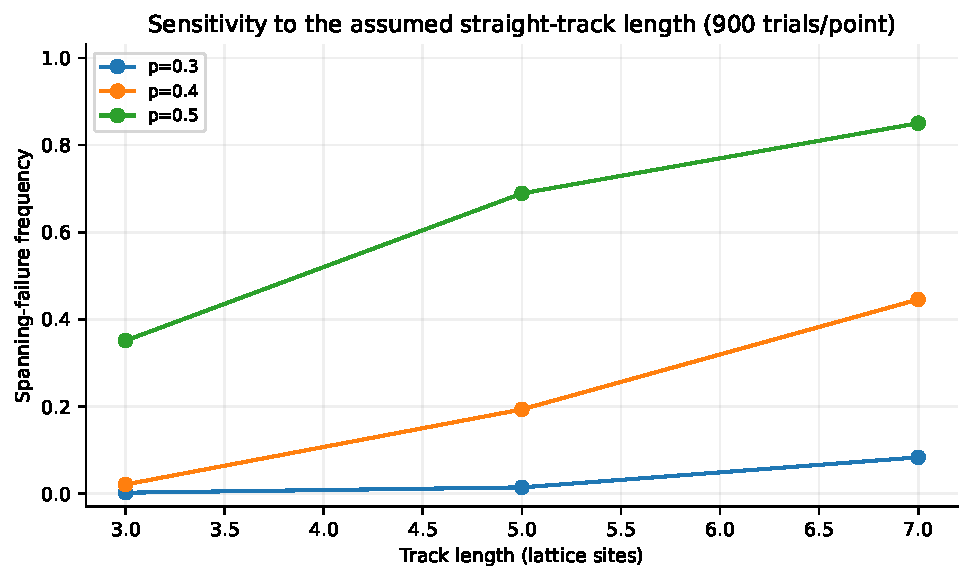
\includegraphics[width=.87\linewidth]{fig09_track_length_sensitivity.pdf}\caption{Sensitivity to finite straight-track length, with occupancy recalibrated for each length. Nine hundred trials are used for each track-length/probability pair.}\label{fig:length}\end{figure}

\subsection{What the benchmark does and does not establish}
The synthetic experiment establishes that, under this declared lattice generator, a matched expected lattice-wide mean occupancy does not imply matched spanning frequency. It also gives a reproducible data set for testing code, plotting, interval calculations, and alternative cluster statistics. It does not show that every correlated process is worse than IID noise. A process that clusters faults in locations that are benign for a particular code could be less harmful than another process with the same mean. It does not estimate a surface-code threshold or holographic-code threshold. It does not simulate DNA damage, lesion chemistry, or repair. It does not infer a physical cosmic-ray rate or biological dose-response curve.

\section{Interpreting the reliability envelope}
\label{sec:translation}
The mathematical layers provide a compact way to state what must be known before a system-level reliability prediction can be made. First, the event process must be characterized. Second, event marks must be translated into a substrate-specific disturbance. Third, recovery and observation must be measured. Fourth, the failure event and horizon must be defined. A statement such as ``the average event rate is low'' addresses only part of the problem.

\subsection{Quantum operating envelope}
For quantum devices, a candidate operating envelope is a set of code/decoder/channel configurations satisfying both logical-risk and real-time constraints:
\begin{equation}\label{eq:quantum-envelope}
\mathcal{A}_Q=\left\{(d,\eta,\tau):P_L(d,\eta;T)\le\epsilon_L,\quad \Pp(\text{decode latency}>\tau)\le\epsilon_\tau\right\}.
\end{equation}
Here \(P_L\) should be measured under event-conditioned channels and include relevant correlations across qubits and cycles. The latency constraint accounts for the real-time nature of fault-tolerant control. The model could include detector-informed mitigation, shielding, material changes, and code/decoder co-design, but those interventions must be evaluated on the same device and benchmark protocol.

\subsection{Biological operating envelope}
For a biological system, an operating envelope might constrain a persistent-lesion endpoint, a chromosome-aberration endpoint, and a viability endpoint simultaneously:
\begin{equation}\label{eq:bio-envelope}
\mathcal{A}_B=\left\{(\zeta,c,\tau):P(L_{\mathrm{persist}}(\tau)>\ell_*)\le\epsilon_1,\quad P(Y_{\mathrm{aberration}}=1)\le\epsilon_2,\quad P(Y_{\mathrm{viability}}=0)\le\epsilon_3\right\},
\end{equation}
where \(\zeta\) denotes radiation-quality and track parameters and \(c\) denotes cellular context. These endpoints should not be compressed into one ``repair success'' value without an explicit measurement model. A cell can repair most measured lesions yet retain a small number of critical lesions; conversely, damage markers can persist without mapping one-to-one to loss of viability.

\subsection{Why matched dose and matched occupancy are different}
Dose matching is a physical exposure design choice. Occupancy matching is a statistical construction in a simplified model. A real experiment could match absorbed dose while observing different track distributions, or match the mean number of qubit error events while observing different spatial correlation. The variables being matched must be stated. For a fair quantum comparison, matching only the average bit-flip rate may still leave different leakage rates and time correlations. For a fair biological comparison, matching dose may still leave different lesion multiplicity and chemistry. In both cases, a richer calibration vector is needed.

\begin{figure}[t]\centering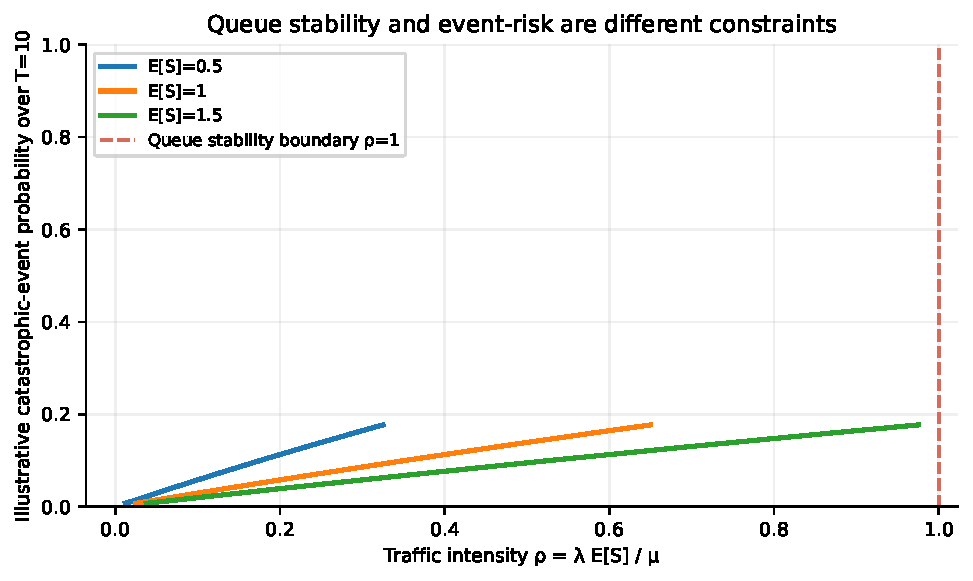
\includegraphics[width=.9\linewidth]{fig10_workload_risk_frontier.pdf}\caption{Illustrative separation of queue traffic intensity and catastrophic-event horizon risk. Curves are dimensionless examples, not fitted device or cell parameters. A stable queue can coexist with a non-negligible catastrophic-event probability.}\label{fig:workload}\end{figure}

\section{Measurement design: from event logs to calibrated kernels}
\label{sec:measurement}
A realistic study should begin with measurement architecture rather than selecting a sophisticated model class. The objective is to capture the event, the induced spatial-temporal response, and the recovery endpoint on a common time base. Without synchronized timestamps and calibration standards, an apparent burst may be an alignment artifact or an unmodeled confounder.

\subsection{Quantum measurement protocol}
A quantum study should collect: (i) radiation detector events with calibrated spatial response and time stamps; (ii) qubit-resolved error or coherence measurements; (iii) device layout and material-stack metadata; (iv) cryogenic operating variables and pulse-tube/vibration channels; (v) stabilizer or syndrome outcomes; and (vi) decoder output and latency. The primary event model should be fitted on one set of runs and evaluated on held-out runs, devices, or operating conditions. Event-triggered averages should be complemented by matched control windows and shuffled-time null models. The analysis should report detector efficiency, event association uncertainty, missing data, and false alarms.

A fair decoder comparison should hold fixed the code family, code distance, syndrome schedule, decoder compute budget, logical observable, and correction deadline. Baselines should include an IID model, a physically motivated correlated model, and an oracle model only when the oracle information is defined and available in the experiment. If a detector signal is used as side information, the latency and resource use of that detector should be counted. A decoder that achieves a lower logical error by consuming information that arrives too late is not an operational improvement.

\subsection{Biological measurement protocol}
A biological study should combine physical track-structure estimates with lesion-sensitive microscopy or molecular measurements and explicit repair time courses. Radiation quality, ion species, energy, dose, dose rate, cell type, cell-cycle distribution, oxygenation, and genomic context should be recorded. Candidate endpoints include clustered DSB foci, lesion complexity, repair-factor recruitment, sequencing-based repair outcomes, chromosome aberrations, and clonogenic survival. These endpoints should be preregistered and analysed separately.

Track simulations can provide a prior for the spatial deposition kernel, but the biological transformation from energy deposition to lesion complexity should be calibrated with empirical assays. Where possible, uncertainty from the track simulator, chemical model, image reconstruction, and cell-to-cell heterogeneity should be propagated into the final repair-workload distribution. A single mean workload is not enough when the tail of the workload distribution drives rare persistence.

\subsection{Calibration, holdout, and falsification}
The validation sequence should be: define an observable; calibrate the event detector; estimate a spatial-temporal kernel on a training set; predict held-out event maps; compare predicted and observed cluster statistics; then evaluate the downstream decoder or repair endpoint. At each layer, a null model and a competing explanation are needed. In quantum systems, vibration and thermal drift are plausible confounders. In biological systems, baseline damage, cell-cycle heterogeneity, oxygenation, and cell-specific repair competence are plausible confounders.

\begin{figure}[t]\centering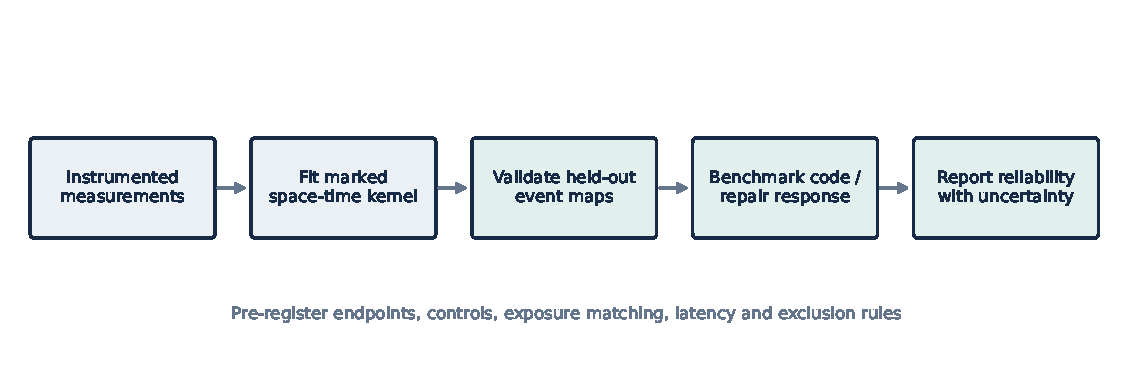
\includegraphics[width=.94\linewidth]{fig11_validation_flow.pdf}\caption{Proposed calibration-to-validation workflow. The pipeline makes the event detector, kernel estimation, holdout evaluation, recovery benchmark, and uncertainty report separate steps.}\label{fig:validation-flow}\end{figure}

\begin{table}[t]\centering\small\caption{Proposed validation programme and minimum controls.}\label{tab:validation}\begin{tabularx}{\linewidth}{p{.18\linewidth}X X}\toprule
Workstream & Core measurement / comparison & Minimum controls and falsification criterion\\\midrule
Quantum burst channel & Detector-synchronized error maps; IID versus event-conditioned decoder at matched marginals & Vibration and thermal covariates; shuffled-event null; reject burst model if held-out predictive calibration fails\\
Holographic code & Explicit tensor/stabilizer code; erased-region correctability; logical error and latency across sizes & Compare with non-holographic baseline; hold decoder budget fixed; no threshold claim without scaling\\
Track structure & Species/energy-resolved kernels; simulated and measured cluster statistics & Track-transport benchmark; dose and geometry records; propagate simulator uncertainty\\
Repair workload & Lesion-class-specific processing-time distribution and repair-factor response & Cell-cycle and cell-type stratification; negative controls; validate workload proxy against independent endpoint\\
Biological consequence & Persistence, chromosome aberration, sequencing outcome, and viability separately & Pre-register endpoints; blinded image analysis; distinguish initial damage from recovery outcome\\\bottomrule\end{tabularx}\end{table}

\section{Adaptive inference and AI-assisted recovery}
\label{sec:ai}
Machine-learning methods can help estimate event-conditioned noise, decode complex syndromes, or allocate limited analysis resources. But an adaptive method should be introduced only after the observation model and control objective are defined. An AI system cannot compensate for an unidentifiable event process or a biased endpoint. It can learn a powerful mapping from data while remaining wrong under distribution shift.

\subsection{Neural decoding under correlated bursts}
AlphaQubit 2 is a neural decoder for topological codes that reports high-accuracy and real-time performance under the noise models and hardware settings evaluated in its study \citep{Senior2025}. Its relevance here is methodological: high-accuracy neural decoding can operate at the timescale needed for error correction, and it motivates testing whether event-conditioned features improve decoding of correlated channels. It does not establish that AlphaQubit 2 is validated on the exact radiation-event distribution in this manuscript.

A suitable experiment would compare decoder variants trained on: (a) IID channel data; (b) event-conditioned synthetic channels; (c) calibrated device-event data; and (d) mixed domains with explicit distribution-shift tests. The main endpoints should include logical error per round, calibration error, worst-case or tail latency, memory, and robustness to event marks not seen during training. Train/test splits must be grouped by experimental run or device where necessary to prevent leakage from temporally adjacent samples.

\subsection{Repair allocation as an optimization problem}
A biological repair-allocation controller can be written abstractly as a constrained stochastic control problem:
\begin{equation}\label{eq:repair-mdp}
\min_{\pi}\E_{\pi}\left[\sum_{t=0}^{H-1}c(X_t,U_t)+\gamma\ell(X_H)\right],\qquad U_t\in\mathcal{U}(X_t),\quad \sum_j u_{j,t}\le\mu_t.
\end{equation}
Here \(X_t\) might encode a measured lesion burden and repair state, \(U_t\) might represent a set of feasible actions, \(c\) a validated resource or damage cost, and \(\ell\) a terminal outcome. This is only a formal problem statement. In a real cell, many repair mechanisms are not directly actuated or even fully observed. The policy class, actions, state, reward, and safety constraints would have to be validated before reinforcement learning is appropriate.

\subsection{Observability and safe exploration}
A central issue is partial observability. A fluorescent damage marker is not the entire lesion state. A detector coincidence is not the complete radiation field. If an adaptive algorithm uses a proxy as though it were ground truth, it can allocate resources to the wrong event class. An offline analysis should first test whether the available measurements identify the state variables used by the proposed policy. In an experimental biological setting, exploration must be constrained by biosafety and ethics review, and no AI-generated schedule should be interpreted as a clinical prescription.

\begin{figure}[t]\centering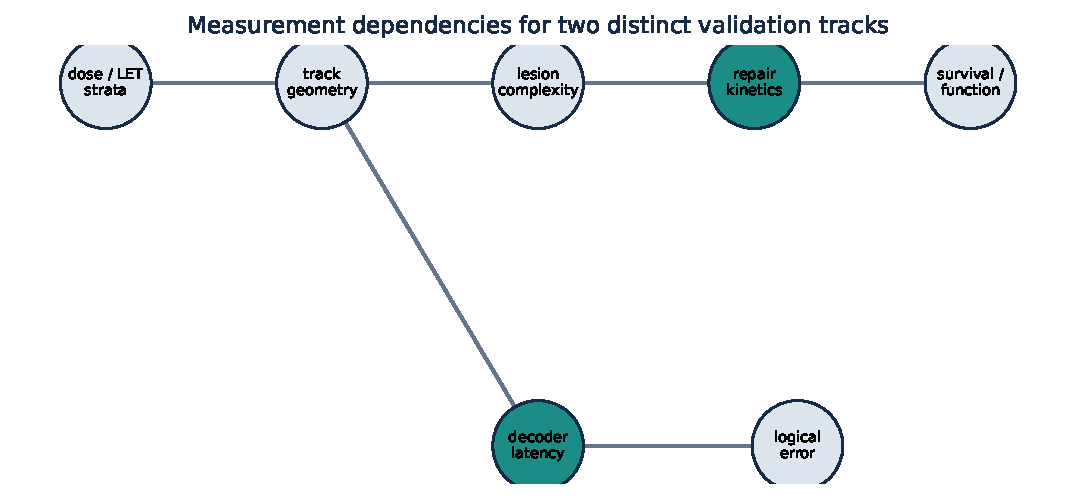
\includegraphics[width=.96\linewidth]{fig12_validation_dependency_graph.pdf}\caption{Measurement dependencies for a cross-domain validation programme. The upper chain represents track and repair measurements; the lower branch shows why decoder latency and logical error belong to a quantum-specific pathway. The graph is a study-design aid, not a causal discovery result.}\label{fig:dependency}\end{figure}

\section{Quantum sensors in living cells: capability and boundary}
\label{sec:quantumbio}
The 2026 Nature study by Abrahams and colleagues reports engineered magneto-sensitive fluorescent proteins, including MagLOV variants, with optically detected magnetic resonance in living bacterial cells at room temperature and single-cell sensitivity \citep{Abrahams2026}. The paper demonstrates a platform for quantum-enabled biosensing and spatial localization, using spin-dependent photophysics associated with a radical-pair mechanism. It is a significant example of quantum measurement in a biological environment.

The correct interpretation is that engineered proteins can support biological quantum sensing. This does not establish that a bacterium is a fault-tolerant quantum computer, that living cells implement holographic quantum error correction, or that the reported sensor repairs radiation-induced DNA lesions. Sensing a magnetic or molecular environment is not the same task as encoding and protecting an arbitrary quantum logical state. The distinction matters because a shared vocabulary of quantum states, noise, or coherence can invite unjustified extrapolation across very different experimental systems.

A possible future cross-domain measurement programme could use quantum sensors to study local environments in cells, while separate radiation and lesion assays quantify track-induced damage. The sensor's own photophysics, excitation conditions, temperature, redox state, and cellular expression would require calibration. The measurement instrument must not be assumed to be a passive observer if its illumination or chemistry changes the cell state.

\section{The neutrino fog: an analogy about inference, not a repair floor}
\label{sec:neutrino}
In direct dark-matter detection, coherent elastic neutrino--nucleus scattering creates a background that can become difficult to distinguish from a weakly interacting massive particle signal. The phrase ``neutrino fog'' describes a statistical inference regime in which additional exposure yields diminishing sensitivity improvements under particular background and signal models. The broader discussion of neutrino backgrounds in next-generation direct detection has been developed for years, including forecasts for the neutrino background in dark-matter searches \citep{Billard2014}. The 2026 XENONnT result reports a measurement of solar \(^{8}\mathrm{B}\) neutrino coherent scattering and discusses the effect of the neutrino fog on dark-matter search sensitivity \citep{XENON2026}. Work such as Blanco-Mas et al. addresses how neutrino backgrounds may still constrain new forces in detector data \citep{BlancoMas2025}.

The analogy in this paper is narrow. In both detector inference and reliability engineering, an observed signal may be obscured by irreducible or poorly separable background processes, and improved exposure alone may not produce proportional information gain. This motivates explicit treatment of background and model uncertainty. There is no claim that solar neutrinos create a biologically relevant repair burden, define a cellular repair floor, or cause the types of DNA lesions discussed in Section~\ref{sec:radiobio}. The neutrino fog is a detector-inference concept, not a biological mechanism.

\section{Limitations, failure modes, and open questions}
\label{sec:limitations}
The framework is intentionally broad, but its components are not yet jointly calibrated. The principal limitation is that the two substrate maps remain external to the synthetic benchmark. The lattice model measures geometric connectedness and does not contain a quantum code or biological mechanism. Its value is to isolate dependence effects under a transparent construction.

\subsection{Model-form limitations}
The track law uses a fixed length, four orientations, uniform anchors, Poisson-distributed event counts, and hard clipping. Physical tracks have energy-dependent radial dose profiles, secondary-electron structure, species-dependent ranges, and stochastic chemistry. A superconducting device's disturbance footprint depends on materials, geometry, phonon transport, quasiparticle dynamics, and measurement circuits. The common mark vector is a placeholder for these richer descriptions. The selected Poisson parent process is not a fit to measured particle arrivals or correlated quasiparticle clusters.

\subsection{Statistical limitations}
The primary sweep has 4,000 trials per point and a finite grid of ten occupancy values. The Wilson intervals account for Monte Carlo binomial uncertainty but not uncertainty about the generator or calibration. The sensitivity runs have smaller sample sizes. The finite-size analysis is too coarse for critical-exponent estimation and should not be read as a percolation threshold result \citep{Grimmett1999}. The extra track-length study changes only one synthetic mark and leaves all other assumptions fixed. The covariance figure is directional and conditional on the chosen track geometry.

\subsection{Queueing limitations}
The M/G/1 result assumes Poisson arrivals, iid service times, one work-conserving server, constant capacity, and no interactions between jobs beyond waiting. Cells have multiple coupled repair pathways and active regulation; decoders are parallel pipelines with finite deadlines, not necessarily single-server queues. A more realistic model may require a vector service network, state-dependent arrival process, time-varying capacity, feedback, or a nonstationary horizon. The stability inequality remains a useful benchmark, but a model should not be selected merely because it gives a convenient closed form.

\subsection{Causal limitations}
A correlation between detector events and qubit observables does not by itself identify all mediating mechanisms. Similarly, a lesion marker after irradiation does not isolate the chemistry, repair pathway, or genomic outcome. Confounding and selection effects must be controlled. Proposed interventions such as shielding, device material modifications, targeted ROS perturbations, or repair-resource allocation are not established by the mathematical framework.

\subsection{Ethical and experimental limitations}
No human or animal data, patient data, live-cell intervention, radiation exposure, or quantum-hardware measurement were carried out for this manuscript. The proposed experimental work would require suitable facility access, radiation safety review, institutional biosafety oversight, ethical approval where applicable, and qualified domain scientists. Synthetic code is not a substitute for those procedures.

\begin{table}[t]\centering\small\caption{Failure modes and the evidence needed to resolve them.}\label{tab:limitations}\begin{tabularx}{\linewidth}{p{.25\linewidth}X X}\toprule
Failure mode & Why it matters & Evidence needed\\\midrule
Wrong event law & Poisson or straight-track assumptions may miss clustering and anisotropy & Detector event records or validated transport simulations\\
Wrong footprint kernel & Equal average burden can hide different spatial dependence & Held-out spatial covariance and cluster-statistic validation\\
Wrong substrate map & Event marks may not translate to errors or lesions as assumed & Qubit-resolved response or lesion-specific assay calibration\\
Wrong recovery abstraction & Scalar capacity omits pathways, parallelism, or decoder deadlines & Service-time data, pathway/network model, latency traces\\
Wrong endpoint & Proxy marker may not predict logical failure or viability & Independent, pre-registered downstream outcomes\\
Overfitted decoder/controller & Strong training performance may not generalize to new bursts & Device/run holdouts, distribution-shift tests, safe evaluation\\\bottomrule\end{tabularx}\end{table}

\section{Falsifiable research programme}
\label{sec:falsification}
The framework is useful only if it makes testable predictions. The following hypotheses are not assumed to be true; they define experiments that could reject or refine the proposed abstraction.

\subsection{Quantum hypotheses}
\begin{enumerate}
\item \textbf{Event-conditioned predictive gain.} A model using detector event geometry and time marks should predict held-out qubit error maps better than an IID model at matched mean error rate. Falsification occurs if the gain disappears under held-out runs or after conditioning on vibration and cryogenic variables.
\item \textbf{Decoder transfer.} A decoder trained on calibrated burst data should reduce logical error or improve calibration under the measured correlated channel without violating latency limits. Falsification occurs if the advantage vanishes under device/run holdout or requires information arriving too late.
\item \textbf{Code geometry dependence.} Different code geometries should exhibit different logical-risk responses to the same measured event footprint. The claim is falsified for a particular comparison if code geometry has no detectable effect within uncertainty under the specified channel.
\end{enumerate}

\subsection{Biological hypotheses}
\begin{enumerate}
\item \textbf{Track-aware lesion prediction.} A track-structure model should predict held-out lesion-cluster statistics better than a dose-only model at matched absorbed dose. Falsification occurs if the track-aware model provides no reproducible predictive gain.
\item \textbf{Workload-tail relevance.} A workload distribution including lesion complexity and pathway-specific processing times should predict persistence endpoints better than lesion count alone. Falsification occurs if the workload representation adds no information beyond simpler predictors.
\item \textbf{Perturbation transportability.} dCas9--KillerRed may calibrate selected localized oxidative damage and repair observables, but transfer to high-LET tracks must be tested and is not assumed. Falsification of transportability is expected if the lesion chemistry, cluster scale, or pathway response differs materially.
\end{enumerate}

\subsection{Cross-domain hypothesis}
A restricted common statistical model may improve forecasting when it preserves event marks, footprint dependence, and recovery workload. It should not be judged by whether the same fitted parameters apply to both domains. The commonality is structural: each domain supplies its own mark distribution, kernel, recovery model, and endpoint. If a shared representation does not improve calibration or predictive efficiency over domain-specific baselines, the cross-domain layer has little practical value beyond exposition.

\section{Conclusion}
\label{sec:conclusion}
Spatially extended events challenge reliability models that retain only an average disturbance rate. This paper sets out a layered mathematical framework in which marked events generate domain-specific footprints, substrate maps convert those footprints into quantum errors or biological lesions, and recovery processes determine whether disturbances become system-level failures. The framework keeps event statistics, physical damage, decoding or repair, and observable-specific reliability separate.

The mathematical results are deliberately modest and explicit. Equal marginal occupancy does not determine a nonlinear failure probability. A standard M/G/1 workload model is stable when its traffic intensity is below one. Poisson thinning gives a closed-form horizon risk when catastrophic marks are independently assigned. These facts can help structure a reliability envelope, but none is a universal threshold for a quantum computer or a cell.

The finite-lattice benchmark reproduces the original 24\(\times\)24 comparison and expands it with exact expected mean-occupancy calibration, uncertainty intervals, covariance and component-size diagnostics, finite-size sensitivity, and track-length sensitivity. Its central observation is specific: under the chosen five-site Poisson line-track generator and four-neighbour spanning criterion, the track process has a higher observed spanning frequency than IID erasures at every tested target occupancy. The correct interpretation is a warning against relying on mean occupancy alone, not an empirical statement about actual quantum or biological systems.

A stronger next study must replace the synthetic track law with calibrated device or radiation-track data, define a concrete holographic or stabilizer code, and validate biological workloads against measured lesion and repair endpoints. Neural decoding and adaptive resource allocation are valuable research directions only after event observability, endpoint validity, latency, and safety constraints have been specified. Finally, the neutrino fog remains an analogy about statistical inference under background limitations in dark-matter detection; it is not a cellular repair floor.

\begin{resultbox}
The defensible conclusion is methodological: reliability under burst-like disturbances is a joint property of event geometry, substrate response, recovery resources, and the chosen failure endpoint. Average error rate, absorbed dose, or mean occupancy alone is generally not enough to identify that joint property.
\end{resultbox}

\appendix
\section{Exact expected-occupancy calibration}
\label{app:calibration}
For a lattice with \(N^2\) sites, there are \(4N^2\) equally likely anchor-orientation pairs in the primary model. For each pair, the five-site segment is enumerated and clipped to the lattice. Let \(c_i\) be the number of anchor-orientation pairs whose segment covers site \(i\). Then
\begin{equation}\label{eq:qi}
q_i=\frac{c_i}{4N^2},\qquad 0\le q_i\le1.
\end{equation}
If the number of independently placed tracks is Poisson with mean \(\lambda_T\), Poisson thinning gives the hit probability \(1-e^{-\lambda_Tq_i}\). The expected mean occupancy is therefore
\begin{equation}\label{eq:meanocc}
\bar p(\lambda_T)=\frac{1}{N^2}\sum_i\left(1-e^{-\lambda_Tq_i}\right).
\end{equation}
The derivative is
\begin{equation}\label{eq:derivative}
\bar p'(\lambda_T)=\frac{1}{N^2}\sum_i q_i e^{-\lambda_Tq_i}>0
\end{equation}
for finite \(\lambda_T\) whenever some \(q_i>0\). Also, \(\bar p(0)=0\), and \(\bar p(\lambda_T)\) approaches the fraction of sites with positive \(q_i\) as \(\lambda_T\to\infty\). In this construction every site has positive cover probability, so the limit is one. Thus each target \(p\in(0,1)\) has a unique nonnegative solution to \(\bar p(\lambda_T)=p\). The code computes it by deterministic bisection to an absolute expected-occupancy tolerance of \(10^{-10}\).

The calibration does not equalize each site marginal. Sites near edges and corners are covered by fewer possible clipped tracks than interior sites. The IID process has marginal \(p\) at every site; the track process has marginal \(1-e^{-\lambda_Tq_i}\). Only the lattice average is matched. This is the correct boundary condition for the specific comparison executed, and it should be stated in every reuse of the result.

\section{Statistical summaries and interval calculations}
For each condition, the estimator of the spanning probability is \(\hat p=k/n\). The Wilson interval at confidence level corresponding to normal quantile \(z\) is
\begin{align}
\tilde p&=\frac{\hat p+z^2/(2n)}{1+z^2/n},\\
 h&=\frac{z}{1+z^2/n}\sqrt{\frac{\hat p(1-\hat p)}{n}+\frac{z^2}{4n^2}},\\
 \mathrm{CI}_{W}&=[\max(0,\tilde p-h),\min(1,\tilde p+h)].
\end{align}
The interval is a binomial sampling interval conditional on a fixed generator and independent Monte Carlo trials. It does not include the uncertainty that would arise from estimating a physical track distribution, choosing a model class, or calibrating the mapping from physical events to faults or lesions. Model uncertainty is likely more consequential than Monte Carlo error in the present stage.

For a zero count in \(n\) trials, the classical rule-of-three approximation gives an upper 95\% bound near \(3/n\). With \(n=4,000\), this is 0.00075. The correct report is therefore ``0/4,000 observed, with a nonzero confidence upper bound,'' not ``the true failure probability is zero.''

\section{Reproducibility and execution protocol}
The main numerical entry point is \texttt{verify\_model.py}. It generates the primary Monte Carlo sweep, finite-size and track-length sensitivity outputs, pair-covariance and cluster-size diagnostics, 12 numbered vector figures and PNG previews, a machine-readable verification report, and standard output. All random generators use NumPy's explicit PCG64-backed default generator through \texttt{default\_rng} and named fixed seeds. The primary results use seed 20261106. Sensitivity analyses use derived fixed seeds so their execution does not alter the primary benchmark sequence.

To reproduce the model in a Python environment with NumPy, Matplotlib, and NetworkX installed:
\begin{verbatim}
python verify_model.py
\end{verbatim}
The report should state PASS, 10 primary probabilities, 4,000 trials per channel and probability, exact expected mean occupancy calibration, and 12 numbered figures. The PDF build is performed from the included \texttt{paper.tex} and \texttt{paper.bib}. The generated PDF page count and rendered-page record are separate checks. Reproducing the synthetic outputs does not reproduce any physical or biological experiment.

\section{Minimum data schema for a future calibrated event record}
A future quantum-device event record should include: event identifier; UTC or synchronized monotonic timestamp; detector identity and position; event class and posterior class probability; coincidence multiplicity; estimated event location and uncertainty; qubit layout version; qubit-resolved response windows; syndrome cycle index; operating temperature and pressure; vibration and pulse-tube features; device materials; decoder version; decoder latency; and all exclusion flags. Raw event times and derived features should both be retained.

A future radiation-track record should include: ion species; kinetic energy per nucleon; LET and its definition; direction; entry coordinate; dose and dose rate; track-structure simulator/version; radial dose profile; secondary-electron statistics; nucleus and chromatin model assumptions; lesion class and multiplicity; assay protocol; cell type and cell-cycle state; repair observation times; endpoint definitions; and uncertainty or quality-control flags. If a lesion workload is inferred, the transformation from lesion class to workload must be documented separately from the physical track record.

\section{Symbol glossary}
\begin{longtable}{p{.17\linewidth}p{.75\linewidth}}\toprule
Symbol & Meaning\\\midrule\endfirsthead
\toprule Symbol & Meaning\\\midrule\endhead
\(\Phi\) & Marked space-time disturbance point process\\
\(Z_k\) & Mark of event \(k\): time, location, orientation, extent, severity, source class\\
\(C(Z_k)\) & Footprint associated with event \(k\)\\
\(K(x;Z_k)\) & Spatial footprint kernel\\
\(G(t;Z_k)\) & Temporal response kernel\\
\(B(x,t)\) & Accumulated disturbance or lesion burden field\\
\(D_t\) & Disturbed or erased set at time \(t\)\\
\(\lambda\) & Parent event arrival rate in a Poisson model\\
\(\lambda_T\) & Mean number of synthetic track placements per lattice realization\\
\(q_i\) & Probability one random track covers site \(i\)\\
\(p\) & Target expected lattice-wide mean occupancy in the surrogate\\
\(S\) & Service workload associated with one event\\
\(\mu\) & Service capacity in work units per unit time\\
\(\rho\) & Queue traffic intensity \(\lambda\E[S]/\mu\)\\
\(q_F\) & Conditional probability a marked event meets a declared catastrophic criterion\\
\(T\) & Observation or reliability horizon\\
\(P_L\) & Quantum logical failure probability for a declared code and channel\\
\(Y_B\) & Biological endpoint, specified per assay\\\bottomrule
\end{longtable}

\section{Research-process disclosure and responsibility}
This work combines a mathematical synthesis, literature review, and synthetic computation. AI-assisted tools were used for research organization, code drafting, literature discovery, and editorial development. The author is responsible for verifying the scientific claims, model assumptions, citations, final manuscript, and release contents. No external peer review, journal acceptance, experimental validation, or DOI deposit is claimed. The manuscript is a public preprint intended to make its assumptions, limitations, and next validation steps explicit.

{\small\bibliographystyle{plainnat}\bibliography{paper}}
\end{document}
